\section{Classification Approach Methods}
\subsection{Forward-Backward Classifier}
In order to learn to classify trips online with minimal hand-labeling of data,
we rely primarily on the forward-backwards classifier approach first proposed by
\citet{spanias2018online} for the purpose of classifying different modes of gait
such as level ground walking, standing, and stair climbing. In their work, a
\emph{forward classifier} predicts the next step's gait mode using data in a
window shortly before the transition. In parallel, a \emph{backward classifier}
labels completed steps with their correct gait mode in hindsight. Because the
backwards classifier has access to features from the completed step, it can
achieve accurate labels with a small amount of hand-annotated data. Once
trained, the backwards classifier can provide labels for training the forward
classifier, obviating the need for further hand-labeling of steps. 

In our work, the forward classifier predicts, shortly after toe-off, if the
upcoming swing will require obstacle avoidance or not. For this purpose, we use
a linear support vector machine and features of the residual limb motion in the
last \unit[210]{ms} of stance and first \unit[90]{ms} of the swing phase.
Because user behavior changes over time in response to changes in prosthesis
obstacle avoidance behavior, we retrain the forward support vector machine every
ten steps using labels from the backward classifier. 

The backward classifier is another linear support vector machine, trained once
for each user, which uses features extracted from the entire swing phase to
label a step as an avoidance attempt after the fact. To train the backwards
classifier we hand label obstacle avoidance attempts and normal steps for
roughly ten obstacles. \Cref{fig:fwd_back} provides an overview of this system.

\begin{figure}[tb]
    \centerline{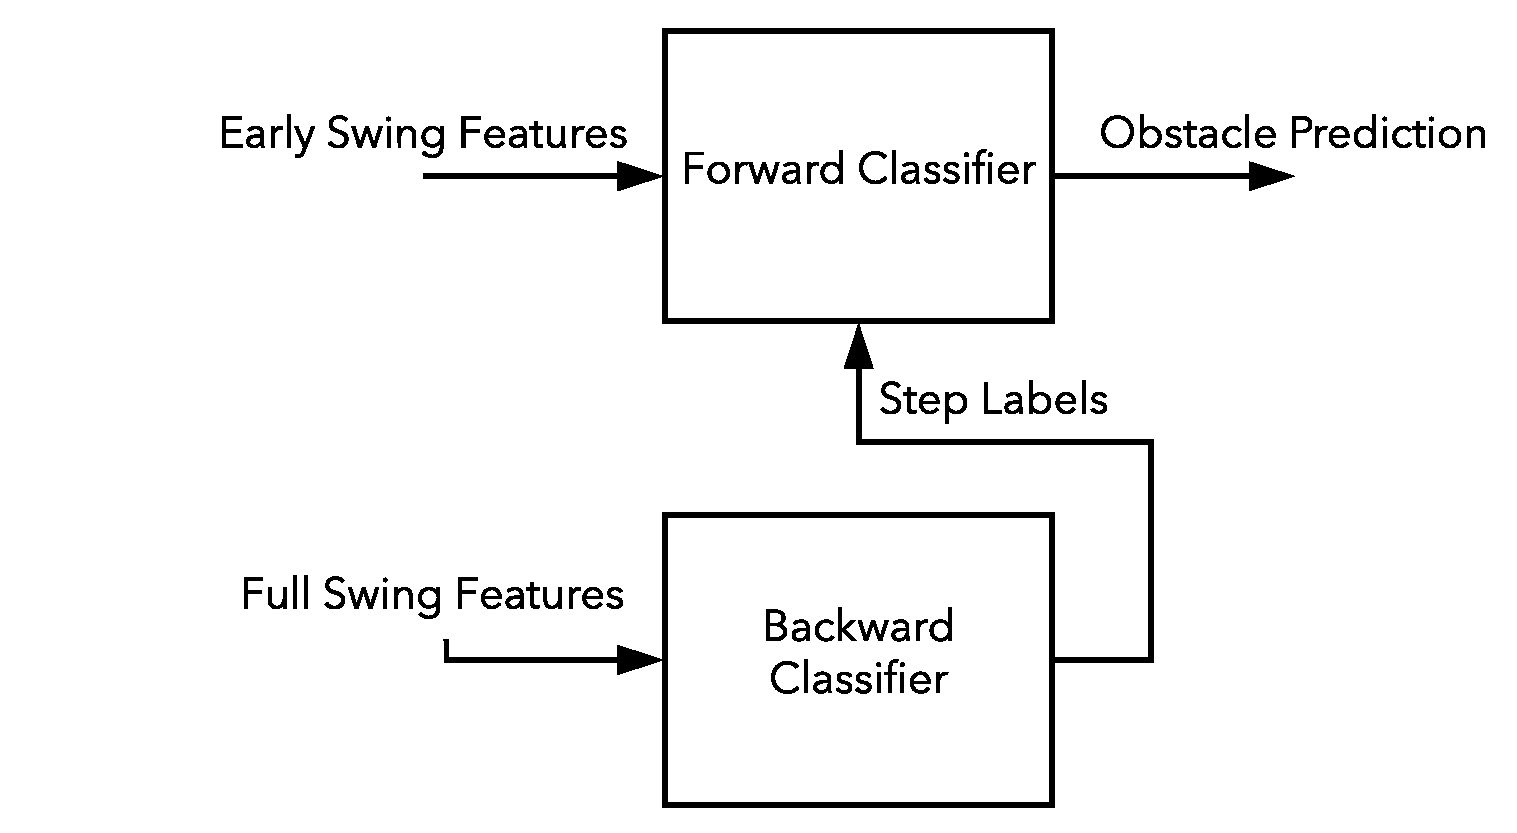
\includegraphics[width=\columnwidth]{Forward-Backward_Block_Diagram}}
    \caption[Forward-Backward Classifier Overview]{Forward-Backward Classifier
    Overview. The backwards classifier uses features from the entire swing to
    provide training class labels to a forwards classifier. The forwards
    classifier uses features from late stance and early swing in order to
    predict if an upcoming swing will be an obstacle avoidance
    attempt.}\label{fig:fwd_back}
\end{figure}

\subsection{Target Knee Angle Regression}

A prosthesis user will not always encounter obstacles of the same height. As the
obstacle avoidance response can be disruptive to the user, it is desirable to
give the user control over the magnitude of the prosthesis response. We seek to
achieve this functionality by using the normalized backward classifier score as
a metric for the difficulty of avoiding an obstacle. We then implement a simple
linear feedback law that assigns higher target flexion knee angles to obstacle
avoidance attempts that are more difficult according to this metric.
\Cref{fig:knee_reg} outlines this feedback mechanism, which has the form
\begin{align}
    \theta_{n+1}^{tgt} &= \theta_{n}^{tgt} - k_\tn{decay}(\theta_{n}^{tgt} 
        - \theta_\tn{min})     + k_\tn{score} \hat{\xi},\label{eq:tgt_angle}\\
    \hat{\xi} &= \frac{\xi - \xi_{10^\tn{th} \ \tn{percentile}}}{
        \xi_{90^\tn{th} \ \tn{percentile}} - \xi_{10^\tn{th} \ \tn{percentile}}},
        \label{eq:score_norm}
\end{align}
where $\theta_\tn{tgt}$ is the current target angle for a given set of features,
$n$ is the current time step, $k_\tn{decay}$ is a gain that prevents continual
target angle growth by decaying target angles towards $\theta_\tn{min}$, and
$k_\tn{score}$ is a gain on the normalized class score, $\hat{\xi}$. The system
shifts class scores, $\xi$, so that scores below the $10^\tn{th}$ percentile of
tripped step scores result in a reduction of the target knee angle. Furthermore,
the system normalizes the scores by $\xi_{90^\tn{th} \ \tn{percentile}} -
\xi_{10^\tn{th} \ \tn{percentile}}$ so that the gain $k_\tn{score}$ has a
predictable effect across subjects whose score ranges vary. 

The system fits the target knee angles with a linear support vector regression.
Every time the trip avoidance triggers, it appends an additional target angle,
specified by \cref{eq:tgt_angle}, to a training data set. The system retrains
the regression using this data set every ten trip-avoidance steps.

\begin{figure}[tb]
    \centerline{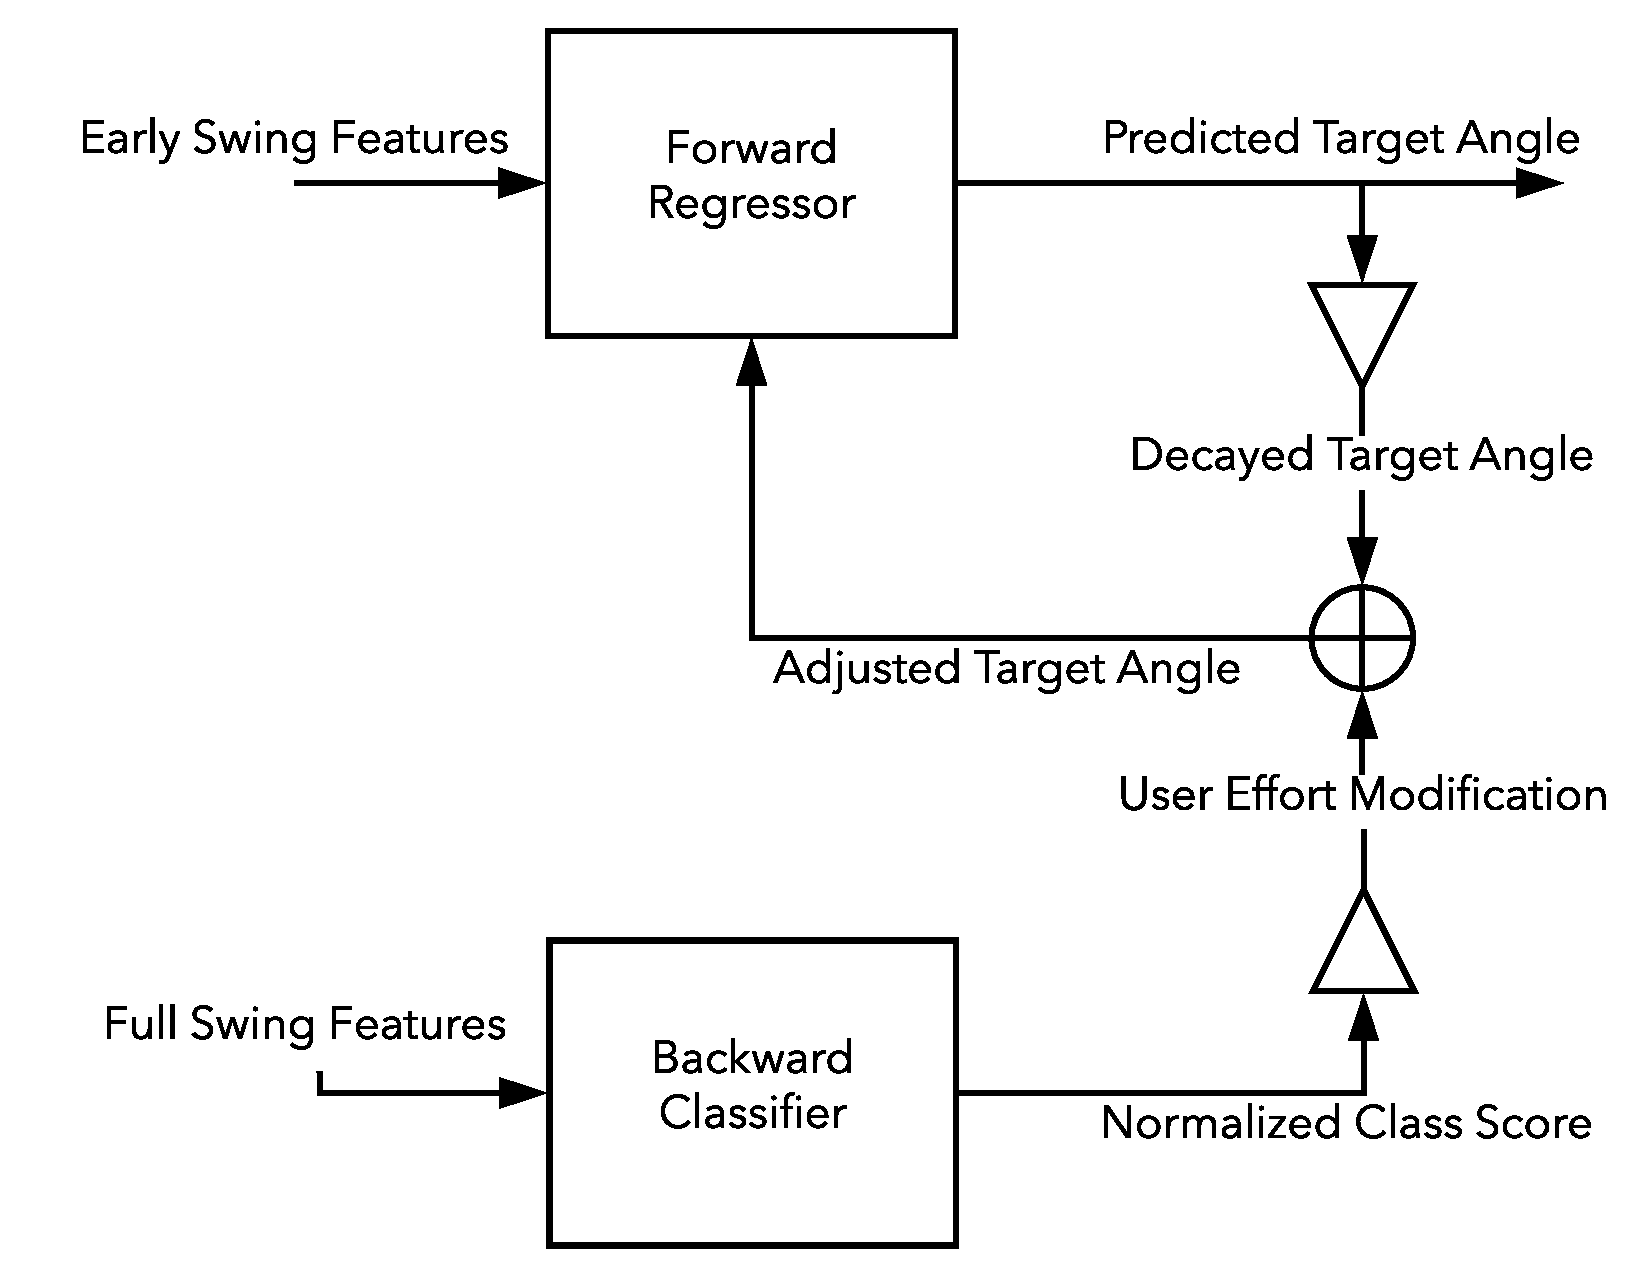
\includegraphics[width=\linewidth]{Regression_Block_Diagram}}
    \caption[Knee Angle Regression Feedback]{Knee Angle Regression Feedback. In
    order to enable volitional control of the knee and ankle flexion angles to
    allow users to achieve greater flexion angles for larger obstacles, we
    implement a feedback system that uses the backwards classifier class score
    to quantify obstacle difficulty. After each step, the system increases the
    desired target angle for that step's forward features proportionally to the
    normalized back classifier score. We also decay the current desired target
    angle for those features to prevent continual growth of the target angle.
    The regression is retrained every ten avoidance
    attempts.}\label{fig:knee_reg}
\end{figure}

\subsection{Feature Extraction}
For the forwards and backwards classifiers, as well as the target knee angle
regression, we use features of the thigh angle, angular velocity, and linear
accelerations in a time window. Specifically, we use the mean, standard
deviation, minimum value, and maximum value of each signal. For forward
classification and regression the time window begins \unit[210]{ms} before
toe-off and ends \unit[90]{ms} after toe-off, while for the backward
classification we use a window consisting of the entire swing phase between
toe-off and heel strike.

\subsection{Trajectory Planning}

To generate the knee and ankle motions for unperturbed swing, we use the minimum
jerk swing control outlined in \cref{sec:nm_control_prosthesis} and first
proposed by \citet{lenzi2014speed}. This swing control scheme  generates and
follows human-like trajectories for the knee and ankle joints that start at the
toe-off angle, angular velocity, and angular acceleration of each joint, go to
target flexion states, and then extend to desired final angles at the estimated
heel strike time. We estimate the swing period to be $65\%$ of the stance
period.

When the forward classifier triggers an obstacle avoidance attempt, we switch to
bang-bang trajectories for the knee and ankle joints. These trajectories
maximize foot clearance while respecting joint angle, velocity, and acceleration
limits. The bang-bang trajectories achieve desired flexion angles as quickly as
possible and then extend as late as possible such that they achieve extension
before the predicted heel strike time. The trajectory planner uses the target
knee angle regression to determine the appropriate peak angle for the knee
trajectory, while the ankle trajectory's target flexion angle is a linear
function of the knee's target angle. The knee trajectory's peak flexion angle is
constrained to lie within 65 and 90 degrees while the peak ankle flexion is
constrained within 5 and 15 degrees. Examples showing the minimum jerk swing
trajectories and obstacle avoidance trajectories planned for large and small
obstacles are given in \cref{fig:avoid_trajs}.

\begin{figure}[tb]
\centerline{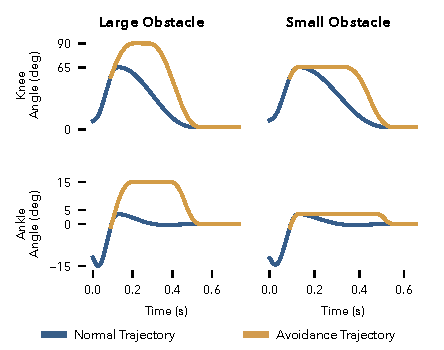
\includegraphics[width=\linewidth]{trajectories_legend}}
\caption[Bang-bang obstacle avoidance and minimum jerk swing
trajectories]{Bang-bang obstacle avoidance trajectories (yellow) vs normal
minimum jerk trajectories (blue) for the knee and ankle.}\label{fig:avoid_trajs}
\end{figure}

\subsection{Experimental Protocol}

We tested the ability of the proposed online learning system to accurately
classify trips and normal swings, help subjects avoid tripping on obstacles, and
modulate knee and ankle flexion appropriately for obstacles of different
heights. To evaluate these aspects of system performance, we conducted
experiments with the powered knee and ankle prosthesis previously described in
\cref{sec:pros_design}.

Two subjects, one non-amputee with prior experience using this prosthesis, and
one inexperienced amputee subject, performed walking trials with the obstacle
avoidance system enabled.  As subjects walked, an experimenter placed objects on
the treadmill belt in front of each subject's prosthetic leg, necessitating an
obstacle avoidance reaction. To obtain a baseline performance level for
non-reactive prosthetic swing control, we also performed obstacle avoidance
trials with the minimum jerk swing trajectories designed for undisturbed swing.
Before the online trials, the backwards classifier was trained for the
prosthesis user with 75 steps. The able bodied subject completed 446 total
steps, with 53 box avoidance steps, while the amputee completed 222 total steps,
with 40 box avoidance steps. The amputee subject performed trials in an ABBA
order, where A is minimum jerk control and B is the reactive control, in order
to average out potential learning effects. The amputee subject also had an
additional practice session the day prior to the box avoidance trials in which
he acclimated to walking with the powered prosthesis without obstacles.
